% !TEX encoding = UTF-8
% !TEX TS-program = pdflatex
% !TEX root = ../tesi.tex

%**************************************************************
\chapter{Contesto}
\label{cap:contesto}
%**************************************************************

%\intro{}\\
Questo capitolo è dedicato all'introduzione delle nozioni emerse dalla fase di apprendimento svolta durante il tirocinio, riguardanti nello specifico le varie di tipologie di DB NoSQL esistenti.\\

%**************************************************************
\section{Cosa significa NoSQL}
Quando si parla di database NoSQL si intendono tutte quelle tecnologie di persistenza di dati che non prevedono strettamente l'utilizzo del paradigma SQL. L'acronimo significa infatti Not-only Structured Query language.\\
Tuttavia, mentre le tecnologie classiche che rientrano sotto l'ombrello dei RDBMS (relational database management systems) sono in qualche modo uniformate dalla "lingua franca" che condividono (SQL), le implementazioni che ricadono nel paradigma NoSQL sono estremamente varie nell'effettivo modo in cui gestiscono i dati, e di conseguenza nei linguaggi che adottano.\\
Questo può rendere il processo di selezione più complesso, ma fornisce anche un'ampia gamma di opzioni che, se scelte con cognizione di causa, possono portare a soluzioni estremamente specializzate ed efficaci.\\


%**************************************************************
\section{Idee e Implementazioni}
Vengono di seguito elencati i vari sottogruppi che possiamo individuare all'interno del panorama NoSQL.\\

\subsection{Key-Value Store}
Questa categoria di DB rappresenta in realtà un modo per immagazzinare informazioni, basato sulla strutturazione dei dati in coppie "chiave-valore".\\
Tutte le operazioni effettuate su un DB di questo tipo si basano quindi sulla chiave per recuperare il suo valore associato. Nella sua forma più semplcie, un key-value store funziona esattamente come un dizionario.\\

\noindent Come esempio abbiamo il caso di Redis.\\
Nasce inizialmente come DB appartenente al paradigma "key-value", composto quindi da un set di chiavi a cui sono legati dei valori, contenuto per intero nella memoria RAM.\\
L'idea era di avere una sorta di cache in cui salvare dei dati frequentemente utilizzati per poterli recuperare molto velocemente.\\
Se inizialmente veniva utilizzato a supporto di altri DB, nel tempo Redis è stato ampliato fino a diventare una soluzione unica (Redis Stack), in grado grazie ai suoi moduli di effettuare ricerche fulltext, visualizzare le informazioni in grafi ed implementare il salvataggio di documenti in formato JSON su memoria persistente in un database distribuito.\\
Il potere di questa soluzione sta nell'avere tutte queste funzionalità all'interno dello stesso prodotto, garantendo una semplificazione non indifferente del processo di integrazione.


\subsection{Wide Column Store}
Questo tipo di database NoSQL estende il concetto di "key-value", dove le informazioni sono raccolte in colonne, le colonne in righe, le righe in tabelle e quest'ultime sono raccolte sotto un cosiddetto "keyspace". A differenza dei database relazionali classici, questo tipo di soluzione non necessita di uno schema, la struttura che definisce il contenuto di una tabella nei RDBMS. Questo permette ai Wide Column DB di accettare dati non strutturati, diventando quindi molto più flessibile.\\
Un'altra importante differenza è che questo tipo di DB è decentralizzato e può essere scalato a dimensioni considerevoli senza troppi problemi, grazie al modo in cui è strutturato.\\

\noindent Prendiamo come esempio cardine il DB Cassandra, che è un database NoSQL distribuito, decentralizzato, scalabile e ad "alta disponibilità". Questo significa che può essere fatto operare su macchine diverse per spezzare il carico, ma soprattutto che non segue il paradigma master-slave. In questo modo tutti i nodi (client) sono omogenei e hanno gli stessi privilegi. La decentralizzazione permette di garantire la disponibilità del sistema, ad esempio quando uno o più nodi dovessero essere irraggiungibili o non responsivi.\\
Si parla poi di scalabilità per gli stessi motivi, poiché aggiungere nodi alla rete e ridistribuire il carico è estremamente facile.\\
Cassandra sfrutta inoltre un linguaggio proprietario simile a SQL, denominato CQL, che risulta quindi facilmente comprensibile se si è abituati a lavorare con DB relazionali.\\

\noindent Questo tipo di DB viene utilizzato quando la disponibilità dei dati 24/7 è una priorità, specialmente se tali dati sono in costante crescita, e la loro struttura tende a cambiare. Il costo da pagare come tradeoff per le potenzialità elencate è una minore consistency dei dati, ma l'argomento verrà approfondito nella \autoref{sec:cap-theorem-integrazione}.

\subsection{Document Store}
Questo paradigma racchiude probabilmente la famiglia più ampia e utilizzata di database NoSQL, presentando comunque soluzioni diverse al suo interno.\\
L'idea principale è sempre quella di non fare uso di uno schema per strutturare i propri dati. Al posto di avere righe in una tabella, in questi DB si usano documents raggruppati in collections. I documenti non seguono una struttura uniforme all'interno della stessa collezione, e sono quasi sempre salvati in formato JSON o simili.\\
In questo tipo di struttura la lettura dei dati è più rapida, a discapito di scrittura e update.\\
Generalmente sono di facile utilizzo e sono tra i DB NoSQL più versatili.\\

\noindent Prenderemo come esempio MongoDB e CouchDB.\\
MongoDB è uno dei DB NoSQL più popolari e diffusi, sfrutta documenti e collezioni, salva i propri dati in formato BSON (Binary-JSON), e adotta il paradigma master-slave.\\
Funziona molto bene quando la funzione principale di cui si ha bisogno è il salvataggio di grosse moli di dati, mentre è meno performante se questi dati devono essere prelevati e rielaborati, specialmente quando è necessario unire dati provenienti da documenti o collezioni diverse.\\
CouchDB è piuttosto simile, sebbene sia un progetto meno popolare. Differisce da Mongo per come salva i documenti (direttamente in formato JSON) e per l'architettura di base, che si distanzia dal paradigma master-slave e sfrutta nodi multipli per mantenere le informazioni sempre disponibili, a discapito della loro consistenza.\\

\subsection{Graph Database}
%Nel panorama dei DB più specializzati annoveriamo quelli basati sui grafi.\\
Esistono alcune categorie di DB all'interno del panorama NoSQL che sono state sviluppate soddisfare necessità specifiche. Una di queste categorie è quella dei DB basati sui grafi.\\
Se nei RDBMS le relazioni sono sfruttate per collegare le tabelle, nel caso dei grafi le relazioni diventano vere e proprie entità, al pari dei nodi che esse collegano.\\
Questo consente di recuperare i dati con richieste (query) più concise e leggibili, oltre che ridurre i tempi di attesa.\\
Questo tipo di DB funziona al meglio in situazioni dove le query si basano molto sulle relazioni tra i dati, dove un DB relazionale dovrebbe operare molte operazioni di Join che aumentano notevolmente il tempo di elaborazione.\\

\noindent Un esempio di DB in questa categoria è Neo4j.\\
Come i DB relazionali, Neo4j è "ACID compliant", ovvero rispetta i parametri di atomicità, consistenza, isolazione e durabilità. Non è tuttavia un database distribuito e soffre quindi quando si parla di scalabilità.\\
Sfrutta un linguaggio molto intuitivo e simile a SQL per le query, chiamato cypher.\\

\noindent Come già detto, questo tipo di soluzione è utile in determinati campi e risulta molto interessante, ma può risultare inutile, o addirittura un ostacolo, se utilizzata in casi in cui non è necessaria.

\subsection{Search Engine}
Un'altra soluzione interessante, ma altrettanto specifica, è quella dei cosiddetti "full-text search engine". Questo tipo di database è piuttosto simile, in superficie, a quelli basati sui documenti, con la differenza che il search engine analizza i contenuti del database e ne fornisce un indice. In questo modo la ricerca di dati, che ovviamente sfrutta tale indice, risulta estremamente rapida anche su dataset molto grandi, con la possibilità di implementare anche vari filtri per migliorare la user experience.\\

\noindent L'esempio più classico di implementazione di questo tipo di tecnologia è Elasticsearch, che è inizialmente nato come search engine e si è successivamente espanso per fornire le funzionalità classiche di un normale database.


%**************************************************************
\section{CAP Theorem, Facilità di Integrazione}
\label{sec:cap-theorem-integrazione}

\subsection{Un altro modo per categorizzare diversi sistemi di archiviazione}
Nel tentativo di categorizzare i DB distribuiti, siano essi relazionali o meno, si sfrutta spesso il cosiddetto CAP Theorem, secondo cui un database distribuito può fornire soltanto due delle seguenti tre garanzie:
\begin{itemize}
    \item \textbf{Consistency}: i dati sono sempre coerenti all'interno dei vari nodi distribuiti;
    \item \textbf{Availability}: i dati sono sempre disponibili in ogni momento;
    \item \textbf{Partition Tolerance}: i dati sono disponibili anche se partizionati, ovvero separati "orizzontalmente" su nodi diversi.
\end{itemize}

\vspace{10pt}
\begin{figure}[htbp]
\begin{center}
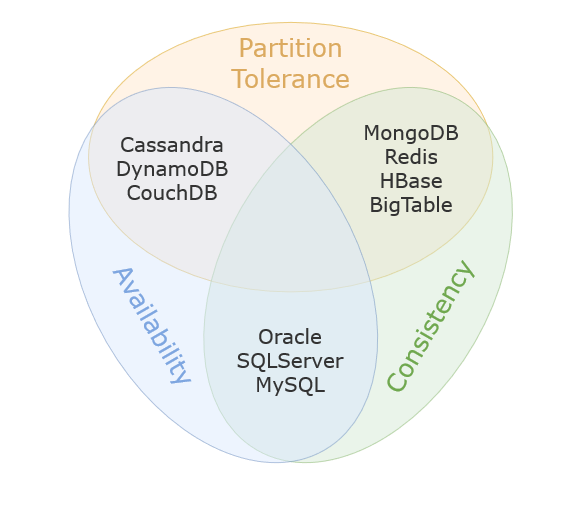
\includegraphics[height=8cm]{cap-theorem}
\end{center}
\end{figure}
\vspace{10pt} 

\noindent Mentre le soluzioni classiche (DB relazionali) garantiscono Consistenza e Disponibilità, ma hanno grossi problemi con la scalabilità orizzontale e la separazione dei dati in cluster diversi, le soluzioni NoSQL tendenzialmente garantiscono il Partizionamento, e possono quindi soddisfare soltanto una delle altre due caratteristiche.\\

\noindent In base quindi alle necessità di Ifin Sistemi, sarà necessario valutare quale tipo di database adottare anche in base al CAP theorem.

\subsection{Integrazione}
Tenendo in considerazione che lo scopo della ricerca che si è condotta rimane quello di studiare la possibilità di integrazione nello stack aziendale, è necessario valutare quanto i database individuati si prestino a tale operazione.\\

\noindent Per ognuna delle implementazioni viste precedentemente è necessario seguire regole specifiche per mettere in comunicazione il proprio applicativo con il database.\\
A volte alcune soluzioni sembrano più funzionali al proprio caso d'uso, ma non hanno un sistema ben documentato/conosciuto/sviluppato per interfacciarsi con l'applicativo che stiamo sviluppando, solitamente per motivi di compatibilità dei linguaggi e diffusione di librerie e driver utili.\\
A tale scopo elenchiamo i software individuati e le loro opzioni di integrazione, tenendo a mente che lo stack aziendale si basa sull'utilizzo di java come linguaggio di programmazione.

\subsubsection{Redis Stack}
Per quanto riguarda Redis, Redis Stack e tutti i moduli ad esso collegati, il modo più semplice e "ad alto livello" per interagire con il database è sfruttare Redis OM, costruito sulla base di Spring Data Redis. Si tratta di un modulo del progetto "Spring Data", che racchiude librerie specifiche per interagire con diversi database usando il framework Spring.

\subsubsection{Cassandra}
Cassandra può essere utilizzato in modo facile tramite Astra DB, un multi-cloud DBaaS costruito su Cassandra.
Per interagire con Astra si possono sfruttare le soluzioni più disparate, dall'utilizzo delle REST API all'implementazione di driver specifici per Java che ne facilitano l'utilizzo.

\subsubsection{MongoDB}
Mongo è una delle implementazioni NoSQL più diffuse e versatili. Si può utilizzare Atlas come "MongoDB as a Service", e anche in questo caso viene fornita la Query API per effettuare operazioni sui dati. Mongo fornisce driver per l'integrazione con Java, ma si può direttamente usare Spring Data, espressamente creato per fornire un modello familiare per datastores basato su Spring.

\subsubsection{CouchDB}
CouchDB non possiede librerie specifiche per l'integrazione e la comunicazione con applicativi scritti in Java. Quelle che esistono spesso non sono ufficiali e quindi utilizzabili "a proprio rischio e pericolo". Risulta possibile implementare la comunicazione direttamente tramite REST API, ma è dispendioso.
Esiste tuttavia una versione di CouchDB sviluppata da IBM, denominata Cloudant, che propone il servizio cloud e l'integrazione con Java.

\subsubsection{Neo4j}
Anche Neo4j ha recentemente fornito una propria piattaforma, lanciando il progetto Aura per fornire DBaaS, con supporto per integrazione con Spring Boot e Spring Data.

\subsubsection{Elasticsearch}
Elasticsearch sfrutta Elastic Cloud come soluzione distribuita.
Possiede varie funzionalità interessanti tra cui la possibilità di migrare i propri dati da un cloud all'altro, a prescindere dal provider.

\subsection{Conclusione della fase esplorativa}
Una volta studiate le opzioni esistenti sul mercato, si è passati alla fase di analisi interna per scoprire quali sono le soluzioni attualmente implementate dall'azienda, come funzionano e quali sono i loro punti critici.

%**************************************************************
\section{Panoramica sui prodotti Ifin e sulle soluzioni RDBMS adottate in azienda}

La seguente sezione è il risultato del dialogo avuto con i team leader di tre diversi gruppi di sviluppo interni all'azienda, necessario per comprendere più nel dettaglio il funzionamento dei software che essa produce e mantiene.\\
Nello specifico, si è ritenuto importante capire quali fossero le tecnologie coinvolte all'interno di questi prodotti, come essi comunichino con i database che sono al centro delle dissertazioni presenti in questa tesi, ed infine quali sono i colli di bottiglia che essi affrontano, per cominciare a farsi un'idea sui punti critici che una migrazione verso un sistema diverso potrebbe migliorare o risolvere.\\

\subsection{LegalArchive}
Il primo prodotto analizzato è Legal Archive, un applicativo che si occupa di archiviazione di documenti con importanza legale.\\
Questo software si occupa di prendere in carico i documenti che un'ente desidera conservare, e tradurli in informazioni che possano essere inserite in un database.\\
Questo è soltanto uno dei suoi scopi, ma è quello che più da vicino riguarda gli argomenti affrontati in tirocinio.\\
Per comunicare con i DB, che in questo caso sono distribuzioni enterprise di Microsoft SQL Server e Oracle Server, LegalArchive si serve di uno stack di strumenti che semplificano tale dialogo.\\
Il database viene montato su un server Tomcat, e per fare uso delle informazioni presenti all'interno di esso si sfruttano il connettore JDBC ed EclipseLink come implementazione della specifica JPA.\\
L'architettura si basa sul pattern Model-View-ViewModel, sfruttando DTO e DAO all'interno del modello per costruire oggetti java derivanti dagli elementi del database.\\
Più semplicemente, ogni elemento di una tabella nel database ha una diretta corrispondenza con un oggetto di una classe all'interno del codice, in modo da poter manipolare tali elementi in base alle necessità.\\
I problemi più grossi che creano rallentamenti nel servizio sono legati alle query utilizzate per richiedere i dati al database.\\
Può infatti capitare che queste vengano testate su campioni troppo piccoli, rischiando poi di dare problemi o "rompersi" quando lavorano sulle grosse moli di dati (fino a circa 200.000 inserimenti di nuove righe ogni ora) con cui il software ha a che fare ogni giorno.\\
Un altro punto critico di questo sistema è il modo in cui si affronta l'aumentare dei dati di cui esso si deve occupare. Finora questo problema è stato affrontato implementando tre diversi approcci di partizionamento:
\begin{itemize}
    \item Partizionamento lato Documenti, dividendo le tabelle più grosse in varie tabelle ordinate con un indice, per facilitarne la gestione;
    \item Partizionamento lato Application, operato sui database da parte dell'azienda;
    \item Partizionamento su diversi database paralleli.
\end{itemize}
Dalle informazioni raccolte emerge quindi come i problemi principali per questo prodotto siano la scalabilità (finora soddisfatta sfruttando vari sistemi di partizionamento delle tabelle) e la rapidità di scrittura e persistenza di nuovi dati.\\

\subsection{InvoiceChannel}
InvoiceChannel è il secondo prodotto per importanza all'interno dell'azienda, ed è strettamente legato a LegalArchive.
Si tratta di un software che fa da ponte tra le aziende ed il Sistema di Interscambio, un servizio dell'Agenzia delle Entrate che gestisce la fatturazione elettronica.\\
TO BE CONTINUED\\
Anche per quanto riguarda Invoice Channel vengono sfruttati sia database Oracle che Microsoft.\\
Sia per quanto riguarda l'ambiente di produzione che negli ambienti dei clienti è presente un'unica istanza, non distribuita nel cloud.\\
Anche IC si basa su Tomcat e JDBC per la comunicazione tra applicativo e database.
Come per Legal Archive, anche per questo applicativo le preoccupazioni maggiori ricadono su scalabilità e performance in condizioni di utilizzo massivo, date le grosse moli di dati in continuo aumento.\\
Anche l'ottimizzazione dei tempi di attesa per determinate operazioni time-sensitive è un tema caldo, su cui si sta ancora lavorando.\\




%**************************************************************
\section{Selezione di un'alternativa}

